\documentclass[tikz, crop, border = {2pt 2pt 2pt 2pt}]{standalone}

\usepackage{concmath-otf}
\usepackage{esvect}
\usepackage{physics}

\usetikzlibrary{calc}
\usetikzlibrary{decorations.pathreplacing}

\begin{document}
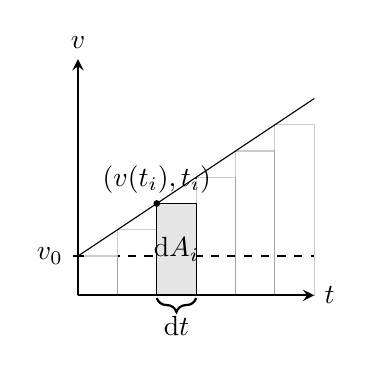
\begin{tikzpicture}[scale = 1]
    \draw[-stealth, thick] (0, 0) -- (3, 0) node[right]{$t$};
    \draw[-stealth, thick] (0, 0) -- (0, 3) node[above]{$v$};

    \foreach \x in {0, 0.5, ..., 2.5} {
        \draw[gray!40, blend mode = multiply] (\x, 0) rectangle ++ (0.5, {0.5+ \x*2/3});
    };
    \draw (0, 0.5) -- ++ (3, 2);

    \coordinate (e) at (1, {0.5 + 2/3});
    \filldraw (e) circle (1pt) node[above]{$(v(t_i), t_i)$};
    \filldraw[draw = black, fill = lightgray!40, blend mode = multiply] (1, 0) rectangle ++ (0.5, {0.5 + 2/3}) node[black, midway]{$\dd{A_i}$};

    % \draw[decorate, decoration = {brace, raise = 1pt, amplitude = 5pt}, thick] (1, 0) -- ++ (0, {0.5 + 2/3}) node[midway, left = 4pt]{$v(t_i)$};
    \draw[decorate, decoration = {brace, raise = 1pt, mirror, amplitude = 5pt}, thick] (1, 0) -- ++ (0.5, 0) node[midway, below = 4pt]{$\dd{t}$};

    \draw (2pt, 0.5) -- ++ (-4pt, 0) node[left]{$v_0$};
    % \draw (1, 2pt) -- ++ (0, -4pt) node[below]{$t_i$};
    \draw[dashed, blend mode = lighten] (0, 0.5) -- ++ (3, 0);
\end{tikzpicture}
\end{document}